\section{Jana Putrle Srdić}

\begin{verse}

\textbf{Věci}

\medskip

Nemá trpělivost se starými věcmi. \\
Když opotřebuje kliku, křeslo, \\
vidličku, větrník, papírové kapesníčky, \\
zahodí je a koupí nové. \\

\medskip

Košíku na houby se to netýká, \\
použitý dvakrát do roka zůstává. \\

\medskip

Knihám také ustoupí, když smrdí \\
vlhkem a plísní, nad nimi nemá moc. \\

\medskip

Květiny občas uschnou, a když je hodí \\
do igelitového sáčku, slyší jejich těla \\
šeptat k~zemi. \\

\medskip

Stoletá skříň v~čerstvě vymalovaném pokoji \\
představuje problém. Její útroby jsou \\
douškem minulosti, který ji vyplivne přežvýkanou, \\
scvrklou jako rozinka, s~vypadanými zuby v~dlaních. \\
Vybaví si své tělo, které se bude nehybně při 1500  \\
stupních proměňovat v~popel, a líbí se jí to. \\

\end{verse}

\podpis{přeložila Hana Mžourková}

\begin{center}
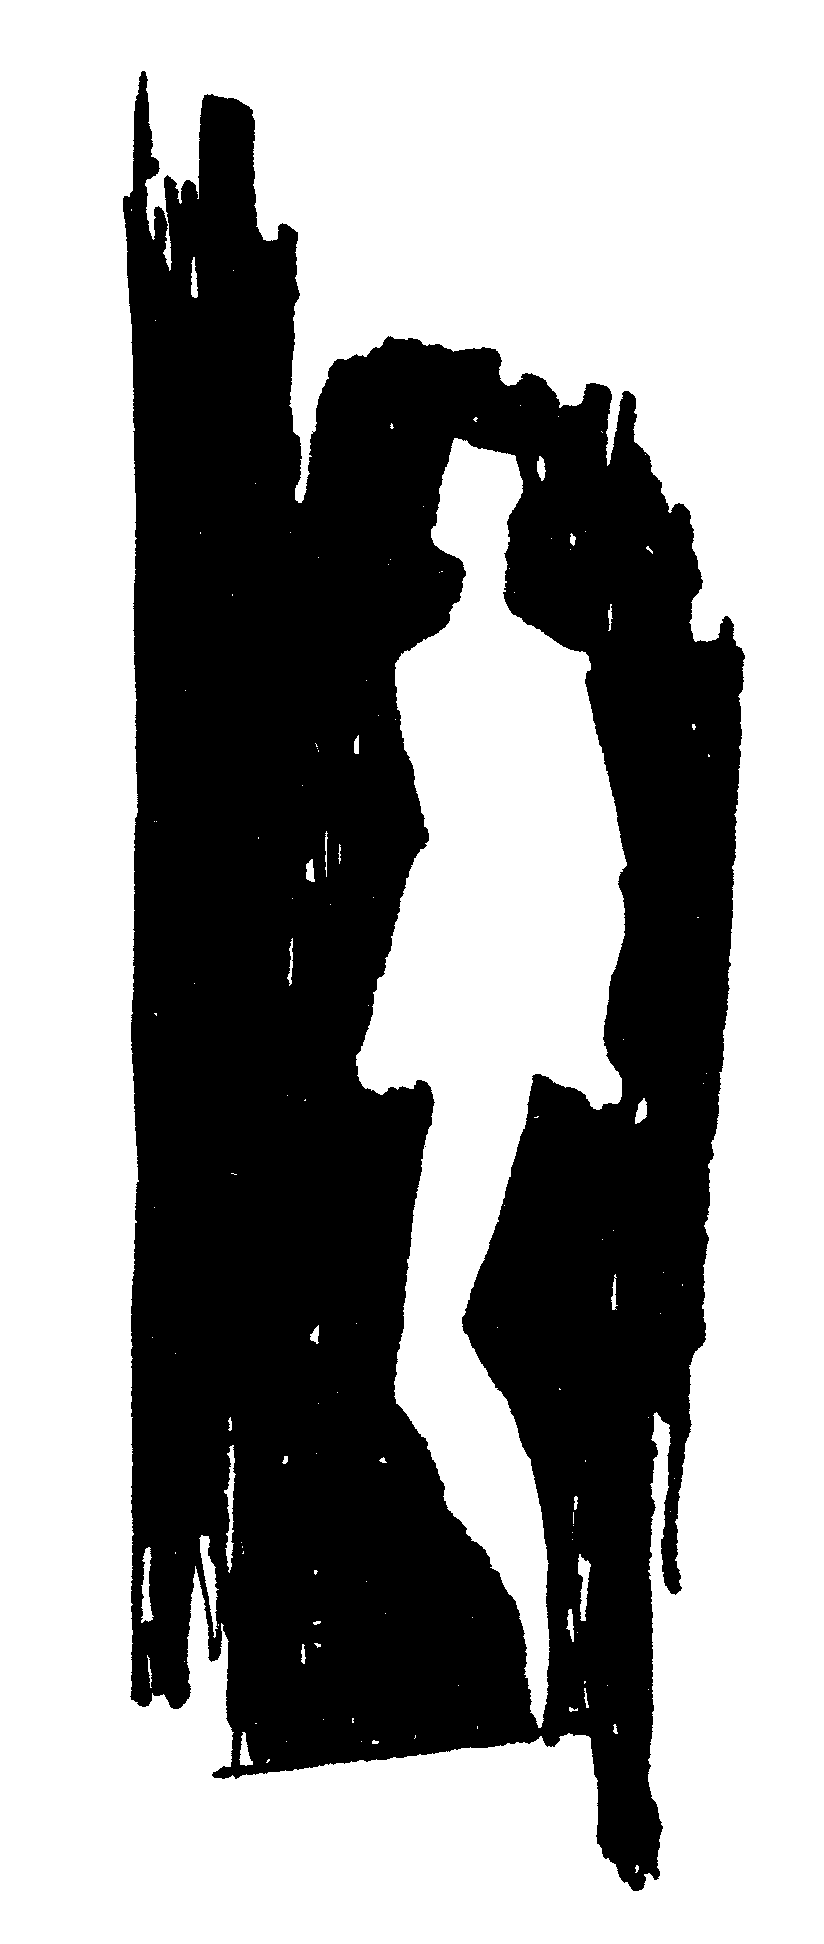
\includegraphics[width=4cm,height=8cm]{plavrevue-30/img/mizen.png}
\end{center}
